\documentclass[english]{tktltiki}
\usepackage[pdftex]{graphicx}
\usepackage{subfigure}
\usepackage{booktabs}
\usepackage{amsthm,amssymb}
\usepackage{amsmath}
\usepackage{url}
\usepackage{paralist}
\usepackage{enumitem}
\usepackage{totcount}

\newtotcounter{citnum} %From the package documentation
\def\oldbibitem{} \let\oldbibitem=\bibitem
\def\bibitem{\stepcounter{citnum}\oldbibitem}

\begin{document}
\onehalfspacing

\title{Analysis of audience engagement and expressed opinion with Data Mining}
% \title{User data analysis with Data Mining techniques}
% \title{Discovering the public's engagement and opinion with Data Mining}
% \title{User data and audience engagement analysis with Data Mining - the case of the Choicely voting platform}
\author{P\'eter Ivanics}

\date{\today}

\maketitle

\numberofpagesinformation{\numberofpages\ pages + \numberofappendixpages\ appendices}
\keywords{data mining, association analysis, user data}

\begin{abstract}
%	1.  What is the problem?
%	2.  Why is this problem important?
%	3.  What does your solution achieve?
%	4.  What follows from your solution?
\end{abstract}

\mytableofcontents

	\section{Introduction}
	\label{section::introduction}
	\subsection{Background and motivation}
    % context, setting - B2C business gathers a lot of data
	Many software businesses collect enormous amount of data generated by end-users. End-user data incorporate essential information about how users interact with the system of discussion as well as tell a lot about the users themselves. Due to the size of the data, a significant part of the information might remain hidden and therefore the business-critical information remains unseen \cite{inmon2007tapping, wegener2010integrating, introtodatamining}. As a result, there is a growing need for all businesses to introduce data analysis processes in their daily activies with the aim of understanding users and their generated data better.  
	
	% what is the potential in analyzing user data? why is it important not only to collect but also analyze data?
	Data analysis tools and methods already exist to help businesses operate on their data. However, these applications often not utilized, because companies rather focus on developing their service package than understanding the previously gathered data \cite{inmon2007tapping}. As a result, essential knowledge concerning previously collected data is neglected, which would be key for the future development of the business. Careful data analysis may reveal interesting relationships and point out facts, what human eyes would never notice otherwise. Consequently, Knowledge Discovery in Databases on user data is important and is essential part of Business Intelligence applications \cite{zarsky2002mine}. 

    % how do mobile devices have an impact on the amount of data? 
    With the continous increase of mobile devices, the amount of data increases significantly. Due to the wide availability and commonness of smart phones and tablets, anybody can easily generate rich location, media or textual data. This fact further increases the call for research in the field of mobile and user data analysis, because it can help researchers to understand the society, human behavior, preferences and public opinions better.

    % what kind of results were derived in the past from end-user data analysis? 
    Depending on the portfolio of the business, analysis of end-user data can reveal various interesting findings. For example, movie databases often contain user reviews on movies, actors and producers of all sort. Such databases are open and are available for the public, and therefore the amount of data has grown huge over the past years. Unsurprisingly, databases like the Internet Movie Database (IMDB) drawn the interest of researchers \cite{saraee2004data, kabinsingha2012movie, sumathi2013performance}. The successful application of statistical methods and data mining techniques on such revealed interesting findings, such as that larger budget does not necessarily result in good ratings by the public, while actors have higher impact on the opinion of the audience \cite{saraee2004data}. On top of deriving such conclusions, machine learning techniques are emerging to predict future movie rating data, based on prior reviews of users \cite{saraee2004data} or the analysis of genre and other attributes of movies \cite{kabinsingha2012movie}.

    % how does researches on social media website data see the user data analysis?  
    Social media data analysis is another trending topic in discovering the secrets of user data. Various researches have applied advanced data mining techniques on Instagram data \cite{jang2015noreciprocity, bakhshi2014faces, hu2014we, jang2016teensengagemorewithfewerphotos, han2016teensarefrommars}, the attached tags and comments added to the images. 

    % why are these researches interesting? What do we learn from the society by performing analysis on user data? 

    % structured and unstructured data is being investigated by different researchers

    % what is the focus? 

    % what is the motivation behind the focus? 

\subsection{Research scope and objectives}


\subsection{Thesis structure}
    % how is the thesis structured? 

    % what is in each of the sections to follow? 

	
	\section{Audience engagement and user data analysis}
	\label{section::audience-engagement-and-user-data-analysis}
	% catch up the thread from the introduction why user data is important
Careful analysis on Big Data can enhance business domain understanding for any company. Accordingly, Big Data has became a widely studied and interesting topic all around the field Information Technology in the recent years, both in scientific and industrial research \cite{inmon2007tapping, introtodatamining}. Significant amount of the data is somehow related to the users of the software at hand. Such data often incorporates essential data about the users themselves, such as their demographic data, preferences or how they interact with the software 
\cite{jang2015noreciprocity, hu2014we, jang2016teensengagemorewithfewerphotos, han2016teensarefrommars, socialdiversityongithub}. 

% how is the term user data used? 
Despite its value and availability, this kind of data is often not looked at, however some interesting studies have been conducted in the field which promotes its analysis \cite{jang2016teensengagemorewithfewerphotos}. Although being widely present, there is no common agreement in the field what user data means. To address RQ1 of this research, user data is defined as follows. 

% what is user data? what does it include or exclude?
The term user data in this study covers two major kind of data that is related to users. On one hand it covers data, which is willingly uploaded and generated by users, on the other hand, it consists of data which generated through interactions while using software solutions (typically online).
% demographic characteristics
The first part of user data typically consists of the demographic characteristics of the users and the content which they have generated \cite{han2016teensarefrommars}. This kind of data often can be found on social media profiles where social demographic information, such as gender, age and nationality are shared.
% digital footprints
Secondly, data gathered during the usage of a software is an important source of information for scientific studies. Researchers use the term digital footprint \cite{youyou2015computer} to describe this kind of data, which composes the second type of user data in this research. Such digital footprints can vary a lot depending on the software of discussion, but typically the include like activities, user comments, photos, posts on social media, ratings in movie databases or browsing history and usage patterns for web browsers. Figure \ref{user_data_venn} demonstrates how user data is understood in this study.

\begin{figure}[h] 
  \begin{center}
    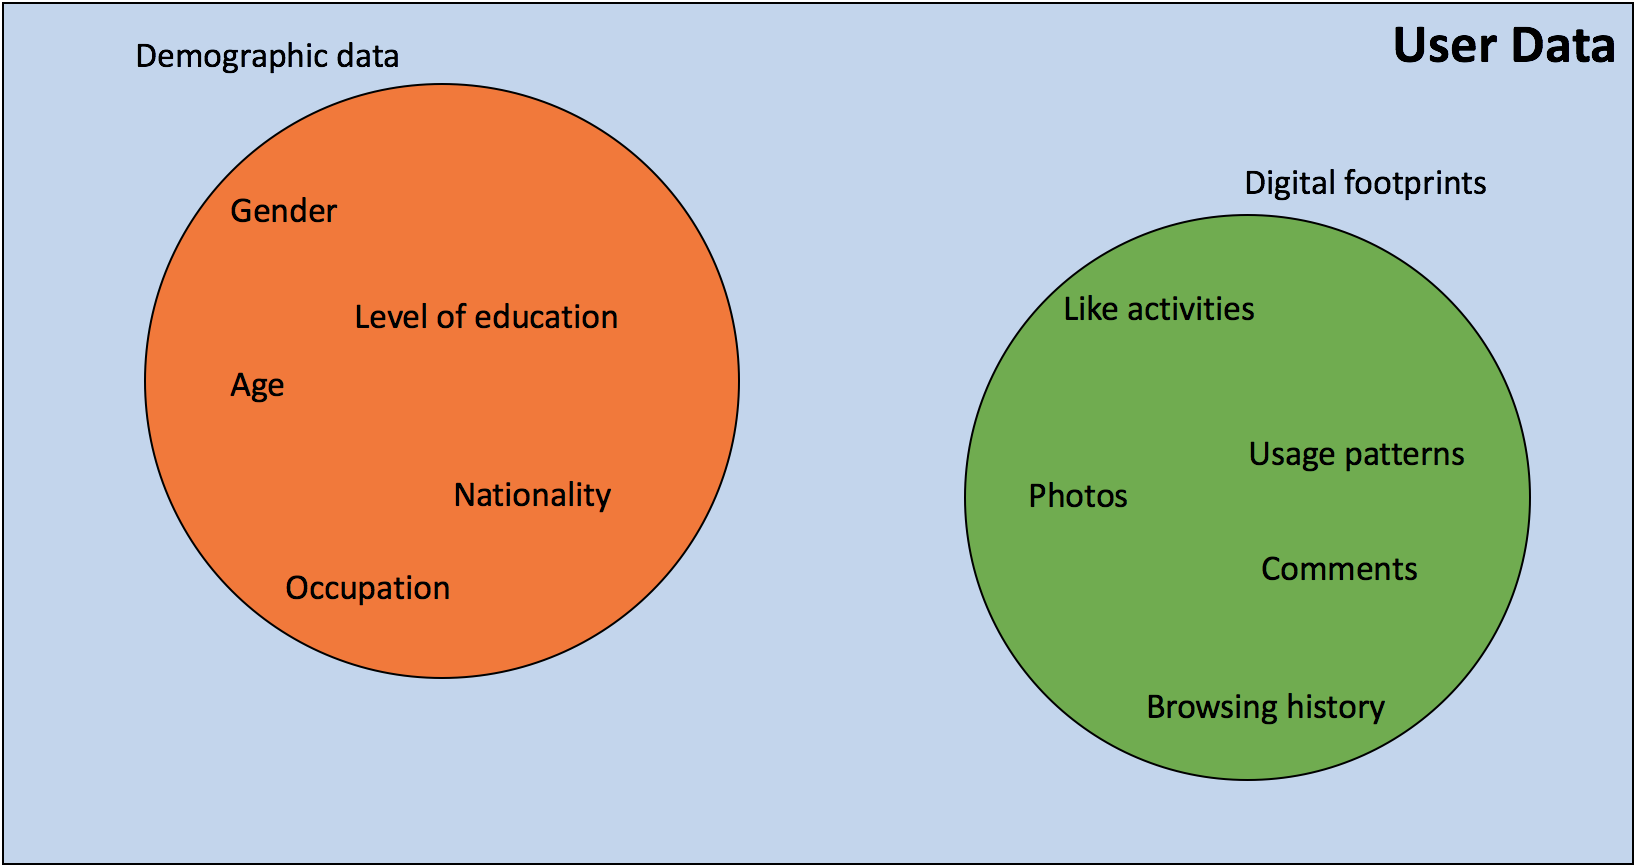
\includegraphics[width=3in]{Images/user_data_venn.png}
    \caption{User data in this research is the combination of users' demographical characteristics and digital footprints.}
    \label{user_data_venn}
  \end{center}
\end{figure}

\subsection{Related research}
% explain that these are often not studied together but rather separately 
The concepts of demographical characteristics and digital footprints are widely studied in the research field, but often only separately, focused on one certain area. Demographic characteristics play a role in analyzing user adoption and behavior, for instance in the banking industry. The study conducted by Wang and Petrounias \cite{chinesemobilebankingusers} reveals that mobile banking in China is more popular among middle-aged males, while the younger generation has not adopted to the new trends yet. By utilizing Big Data analytics the group of citizens and products for the upcoming marketing campaigns were revealed \cite{chinesemobilebankingusers}, which greatly enhances the marketing activities of financial organizations. Social diversity was also studied by other researchers in the context of software development growth \cite{socialdiversityongithub}. In their study, Aué et al. \cite{socialdiversityongithub} have clearly identified correlation between the success of open source projects and the contributors' gender and cultural diversity by utilizing well chosen statistical methods. 

Like activities performed on social media are widely studied concept \cite{bakhshi2014faces, jang2015noreciprocity, jang2016teensengagemorewithfewerphotos, ottoni2013ladies}. Comments, hashtags and content that is generated by users are also widely studied \cite{bakhshi2014faces, jang2016teensengagemorewithfewerphotos, hu2014we, bakhshi2014faces} and also contribute to this kind of data in this study. However, little research has been conducted in the field on how these usage patterns can be projected onto demographical data, which can greatly contribute to understand user behavior of certain target groups. Despite the fact the term user behavior is widely studied, researchers claim that its concept is used rather ambiguously \cite{waheed2017investigation}.
%Furthermore in case of social networks, the users' contribution to the available content is essential, which is often called as user-generated content (UCG) \cite{jang2016teensengagemorewithfewerphotos}. 

% what kind of results were derived in the past from end-user data analysis? 
Movie databases often contain user reviews on movies, actors and producers of all sort. Such databases are open and are available for the public, and therefore the amount of data has grown huge over the past years. Unsurprisingly, databases like the Internet Movie Database (IMDB) has drawn the interest of researchers \cite{saraee2004data, kabinsingha2012movie, sumathi2013performance}. The successful application of statistical methods and data mining techniques have revealed interesting findings, such as that larger budget for movies does not necessarily result in good ratings by the public, while actors have higher impact on the opinion of the audience \cite{saraee2004data}. On top of deriving such conclusions, machine learning techniques are emerging to predict future movie rating data, based on prior reviews of users \cite{saraee2004data} or the analysis of genre and other attributes of movies \cite{kabinsingha2012movie}.

% how do researches on social media website data see the user data analysis?  
Social Networking Sites (SNSs) are another trending source in discovering the secrets of user data as the number of scientific publications in the topic has increased significantly in the recent years \cite{waheed2017investigation}. Various researches have applied advanced data mining techniques on Instagram data \cite{jang2015noreciprocity, bakhshi2014faces, hu2014we, jang2016teensengagemorewithfewerphotos, han2016teensarefrommars}, more specifically on the tags and comments that are attached to the images. Similarly, like activities and user-generated content is studied by the scientists. It is revealed, that Instagram users can be divided into two groups based on their activities: specialists, who publish and seek content around a certain topic of interest; and generalists, who are interested in all kinds of genres in the social media site \cite{jang2015noreciprocity}. Data mining techniques also allowed researchers to conclude, that the teenager users of Instagram tend to be more active, faster to react and more open to communicate with other users on social media \cite{jang2016teensengagemorewithfewerphotos, han2016teensarefrommars}. Furthermore, it was discovered that media content with human faces are more engaging than other type of media \cite{bakhshi2014faces}. Finally, rich social media data allowed researchers to analyze behavior and user preferences among genders, age groups and locations \cite{farseev2015harvestingmultiplesources}.

% facebook reactions
Recently Facebook has introduced reactions among their features. Through reactions, users can not only "like" content, but also express other emotions, such as love, joy, amazement, anger or sadness \cite{shouldfacebookusereactions, howarenewspublishersreactingonfacebook}. This way users' emotional feelings about the content can be collected easily and efficiently. Shortly after its release, it was identified that the new feature is very popular and generally engages a wider audience than previous likes and comments \cite{shouldfacebookusereactions}. Study also shows, that reactions are a great way for publishers to get a feedback on the public's opinion \cite{howarenewspublishersreactingonfacebook}. On top of that, reactions offer an easy way for content providers to organize a by assigning one of the available reactions to the participants and asking the users to react on the content with their favorite's reaction \cite{shouldfacebookusereactions}. The limitation on such polls is that users have the possibility to choose only one of the reactions and hence only one of the participants as their answer to the voting.  

% where is all this research coming from?
Interestingly, most of the SNS-related studies are conducted in the United States of America and Asia \cite{waheed2017investigation}. Only a few studies were conducted in the European region, which allows to conclude that there is a great interest and development possibility in the area. However it is important to highlight, that due to the wide popularity of the international social networks (such as Facebook, Instagram or Pintrest), some part of the data may be derived from users in the European continent. It was also pointed out that some researches focus on sites, that are specific to a particular region or country \cite{waheed2017investigation}, which means the findings are strongly related to the cultural environment of the user base.    

% what does user data analysis reveal in a corporate social media environment? [refer to \cite{guy2016whatsyourorganizationlike}]
Social media platforms in enterprise environment are studied similarly to regular social networks \cite{guy2016whatsyourorganizationlike}. Despite the fact that the two types of social media platforms share many features, analysis performed in enterprise environment can provide great insights about how employees interact and cooperate. Among many other findings, studies have shown that blogs posts in an enterprise social media site tend to be more engaging and contribute to form communities inside the organization \cite{guy2016whatsyourorganizationlike}. Such insights are essential for higher management, because it can be used for instance to identify departments that tend to be less interactive or engaged.  

\subsection{Tools and methods}
Various methods were utilized in previous research to arrive at the the findings above. The major types of the techniques and their purposes are explained in the paragraphs to follow. Table \ref{table_of_techniques} below lists the same findings.

% what methods are utilized? 
  % multiple data sources
   The combination of multiple data sources, such as Facebook, Instagram, Pintrest or other social media profiles via their connection is a common practice in researches \cite{farseev2015harvestingmultiplesources, ottoni2013ladies}. Researchers have managed to perform complete demographic profiling and concluded that the intergration of multiple data sources is indeed a great method of enhancing performance on user data analysis \cite{farseev2015harvestingmultiplesources}. 
  
  Utilizing additional tools, existing datasets can be further enhanced for data analysis purouses. A great specimen for this is computer vision, which is used in numerous studies to identify content of photos \cite{hu2014we, farseev2015harvestingmultiplesources}. In another study, similar techniques are utilized to identify faces on and predict ages of people from photos on social media sites \cite{han2016teensarefrommars, bakhshi2014faces}. Through these reserches, computer vision is proven to be a powerful tool to facilitate the information in the data and can provide researchers further data for their studies. 

  % text processing techniques
  Text processing techniques are potentially the most common way to discover the insights of user data. The Linguistic Inquiry and Word Count (LIWC) and Latent Dirichlet Allocation (LDA) methods are used by researchers \cite{ottoni2013ladies, farseev2015harvestingmultiplesources, jang2016teensengagemorewithfewerphotos} for extracting linguistic features of text, identifying keywords in comments and reviews as well as for topic modelling on user comments, reviews or hashtags on Instagram. Topic modelling was also applied for analyzing genres of movies by their title and description \cite{kabinsingha2012movie}. Applying natural language processing techniques also allowed researchers to infer age and gender of users \cite{han2016teensarefrommars} who have commented on content on Instagram. Utilizing these methods greatly contribute to the undertsanding of data gathered, which can lead to richer analysis and pattern recognition on the dataset at hand.
   
  % supervised ML techniques
  Supervised machine learning is often used for prediction tasks performed on user data. Decision trees are often utilized as prediction tools for the purposes of identifying audience of mobile banking software in China \cite{chinesemobilebankingusers}. Decision trees were also successfully used for movie rating prediction \cite{saraee2004data} and classificiation of movies \cite{kabinsingha2012movie}. Bayesian networks in the same study \cite{kabinsingha2012movie} are also investigated and are found as the most suitable method for predictions in the area of movie ratings. Ensemble Modeling, which is another supervised learning method, is successfully used for user profile learning on social media sites \cite{farseev2015harvestingmultiplesources}. Similarly, Support Vector Machines and Logistic Regression was utilized for predicting age group of users based on their social media activities \cite{han2016teensarefrommars}. Last, but not least Negative Binomial Regression is put in use to model like activities in researches \cite{jang2015no, bakhshi2014faces}.

  % unsupervised learning - less popular but still possible
  Unsupervised machine learning techniques are present in the literature. As an example, clustering is used by Saraee White and Eccleston \cite{saraee2004data} for detecting relationships between the ratings given on a movie and the year it was published. In another study \cite{hu2014we}, the k-means algorithm was used successfully to create five clusters of Instagram users based on the type of content they have uploaded to Instagram. These results share similarities with another study \cite{jang2015no}, where generalist and specialists groups were identified based on their like activities based on natural language processing techniques. 

% frequent itemset
Frequent Itemset Analysis is utilized by Ottoni et al. \cite{ottoni2013ladies} for user portfolio analysis and detecting differences among genders in their data. By utilizing this technique, the researchers have identified significant differences between the two genders' preferences in terms of online content \cite{ottoni2013ladies}. 

\begin{table}[!t]
  \centering
    \begin{tabular}{c||c}
      Technique & Number of studies \\ 
      \hline
      Computer vision & 3  \\
      Text processing & 5 \\
      Unsupervised machine learning & 2 \\
      Supervised machine learning & 5 \\
      Frequent Itemset Analysis & 1
    \end{tabular}
    \caption{The summary of utilized data mining techniques on user data in other researches.}
    \label{table_of_techniques}
\end{table}

\subsection{Conclusions} % TODO maybe summary instead of conclusions? 
% why are these researches interesting? What do we learn from the society by performing analysis on user data? 
The examples in the previous chapters demonstrate the relevance of Data Mining and Machine Learning methods in the field of user data and demographic analysis. The proper application these methods allow us to learn more about the society as well as human behavior, which was not possible in the past. This information is essential for business operations, because it gives insights on the user groups, their preferences and what kind of content keeps the audience engaged. 

From the chosen set of related studies it seems, that natural language processing and supervised machine learning techniques are the most common approaches for conducting research on user data. The encouraging results achieved by other researchers prove the relevance of computational techniques applied on user data in a wide range of development areas, such as banking, social media, online movie databases, user portfolio analysis to name a few. Despite not being part of this short study, recommender systems could be an interesting topic of further development and discussion in the area.  

In the past these kind of insights were unavailable to researchers and content providers. In the present time, access to this information can facilitate research, business processes, helps determining the future content, analyzing trends and understanding target groups of particular services better. In sum, modern data mining techniques created the potential to study human preferences and behavior from a different angle.

% how does all of this relate to the rest of this research? 	

	% \section{Data mining}
	% \input{data-mining}
	
	\section{Data mining at Choicely}
	\label{section::data-mining-at-choicely}
	This chapter explains the Data Mining tasks that are introduced at Choicely through this thesis work. The first subchapter introduces setting in which this research is conducted. The reason behind this is to provide more insights over the introduction presented in Chapter \ref{section::introduction-to-the-choicely-voting-platform}. Secondly, learning about the system's core functionality related to this research provides a better understanding for the rest of this study. The second subchapter introduces relevant insights on the company's data related ot this research. Finally, the last subchapter argues for the relevance of the selected methods and explains how they are applied in this study. 

\subsection{The voting mechanism and the user profiles}
% voting options
Various voting options are available for Choicely contests. The author of the contest has the choice of setting a limit on how many votes users can spend on individual participants or the whole contest in overall. For instance, if the maximum votes in the contest is set to 1, users can give exactly one vote on one and only one participant. Configuration settings allow infinite votes as well. For instance, users may vote on all of the participants as many times as they like in a talent show in this case. Removing votes is possible, if the author has decided to enable this possibility. Votes cannot be modified after the contest has ended. Each contest has its own voting configuration. 
    
% free-silver-gold votes
On top of the regular free votes, contest authors may allow users to earn more votes (called "silver votes") by sharing the contest on social media or by watching advertisements. Furthermore, contest authors can allow users to purchase more votes (called "star votes" or "gold votes") with exactly the same restriction settings as explained above. Note, however that the configuration for the three vote types are distinct for every contest. This means that the limitation on free/silver/star votes may differ for individual participants as well as the whole contest. For instance, a contest author may allow users to spend only 5 votes for free, but unlimited number of silver and gold votes in a contest. 

In this research, there are no distinctions made between the different vote types. That is, free, silver and star votes are considered as equal. The rest of this study makes no difference between the different vote types, but simply considers them as votes on contest participants, which is a sign of favor shown by the user towards the contest participants. Nevertheless, it would be interesting to separately study if there is any significant difference in how users spend different types of votes. 

Each user profile contains the features listed in Table \ref{user_profile_fields}. For the purposes of this research, the fields written with blue text are considered interesting part of user profiles. The three highlighted attributes are all categorical variables, that contain demographic information about uesrs. By filtering the data using these demographic attribues, one can obtain data generated by targeted segments of users and compare those datasets. This way the behavior of the demographic groups can be studied, which provides answer to RQ3. To keep the scope of this research compact, only the country information of the users is utilized in this study.

\begin{table}[]
    \centering
    \begin{tabular}{l|l}
        \textbf{Field}              & \textbf{Type} \\
        \hline
        Full name                   & Free text \\
        Profile picture             & Image \\ 
        Cover image                 & Image \\
        \textcolor{blue}{Gender}    & Male/Female/Not chosen \\
        \textcolor{blue}{Location}  & Country, state and city \\
        Birthday                    & Datetime \\ 
        \textcolor{blue}{Age group} & 0-17/18-24/25-34/35-44/45-54/55-64/65+ \\
        Introduction/Bio            & Free text
    \end{tabular}
    \caption{The list of fields and their types for each user profile.}
    \label{user_profile_fields}
\end{table}  

The demographic data is filled by the users at the time of signing up for the service. Contests require users to have a user profile in the Choicely platform. Choicely offers authentication through social media (Facebook and Google+) as a convenient option for users to sign up with one click. In this case, the social media platform provides information about the user's profile to Choicely, which allows the automatic population of the demographic data of the user. Optionally, user profiles in Choicely can be created through a regular sign-up process, where users pick a username as their identities. In such case, their demographic data is unknown by default and it is up to the users to complete their profiles. 

% what kind of data is generated?
In sum, the user data in Choicely is two-folded: the user profiles contain demographic information about the users, namely age group, gender and location. Contests have a number of participants with arbitrary number of votes that the users have already casted. The latter kind of data can be seen as digital footprints generated by users in the Choicely platform. The combination of these datasets sums up to the user data as explained in the previous chapter and Figure \ref{user_data_venn} in this particular case. This is further supported with the meta data of contests explained in the previous paragraph. 

\subsection{Research setting}
    % why is the data analysis relevant from scientific research point of view?
    Performing scientific research on such data is interesting for multiple reasons. To begin with, at the time of this research Choicely did not utilize data analysis tools on the collected data. It is in the interest of the company and its customers to better understand what kind of audience was engaged in the past, what kind of content is more (or less) successful and what tendencies in user behavior can be extracted from the data. By doing so, both parties can provide better services and richer content to their targeted customers. Therefore, the introduction of data analysis and visualization tools at the company will greatly enhance business value of the firm, provide deeper understanding on the domain as well as the existing user base.   
    
    % how is Choicely different than other social networks or any other repository of user data?
    Secondly, Choicely can be looked at as a social network, because some of the pictures uploaded to the platform is generated by users. Users also have the possibility to express their appreciation or support towards some contest participants by spending votes on them. Similarly to social networking sites, where the "like" feature is often used \cite{jang2015noreciprocity, bakhshi2014faces} this phenomena can be looked at as a way of expressing personal opinion. 
    
    In comparison to most of the currently available social networks, voting platforms like Choicely are observed by the audience differently. On one hand, social media sites usually list posts or images on a feed, where there is theoretically no relation between the posts that follow eachother. % TODO citation
    On the other hand, contestants in the Choicely platform share similarities as they were nominated for the same contest. Accordingly, there must be some similarity among them as all are subjects of the contest's topic, rules and are competing for the best possible result. 

    % so what? Why is that important from user point of view
    This slight difference can make a big change in terms of user behavior. The focus moves from "what kind of content I like" to "which piece of content I like the most in comparison to the rest". Consequently, users will scan through some (or optimally all) of the contestants and make unconscious decisions upon whether to give vote(s) on certain contest participant(s). The users express their favour and support towards a subset of contenders, hence helping them to reach their ultimate goal: winning the contest. 
    % how can this contribute to user behavior and social media studies? 
    This uniqueness compared to other social networking sites offers a great possibility for research. Therefore, the hands-on goals towards the analysis are two-folded: 

    \begin{enumerate}
        \item identifying what kind of images among different contests users like, and
        \item what kind of content similar group of users like.
    \end{enumerate}

    % how computer vision is going to be utilized? 
    One of the challenges in connecting users with topics is that there is no indication on what the content on the participants' pictures is. Contest authors only assign categories to the contests to be created, which does not necessarily describe the entrants. Other researches have successfully utilized computer vision to gather meta data for the uploaded content in image sharing communities \cite{bakhshi2014faces, hu2014we}. 
    
    % what is the solution to this problem?
    Deriving from the success in previous studies \cite{hu2014we, farseev2015harvestingmultiplesources, han2016teensarefrommars, bakhshi2014faces}, computer vision is applied in this research to identify labels that appear on the participants' images. For instance, a beauty pageant's entry image may be labelled with meta data, such as "Beauty", "Photo Shoot", "Smile" and "Blonde". Similarly, a design contest entry might have topic labels, such as "Landmark" or "Architecture". Figure \ref{google_vision_labels} displays an example, where the Google Vision API was used to extract labels from images which were used in contests of Choicely.

    \begin{figure}[h] 
		\begin{center}
            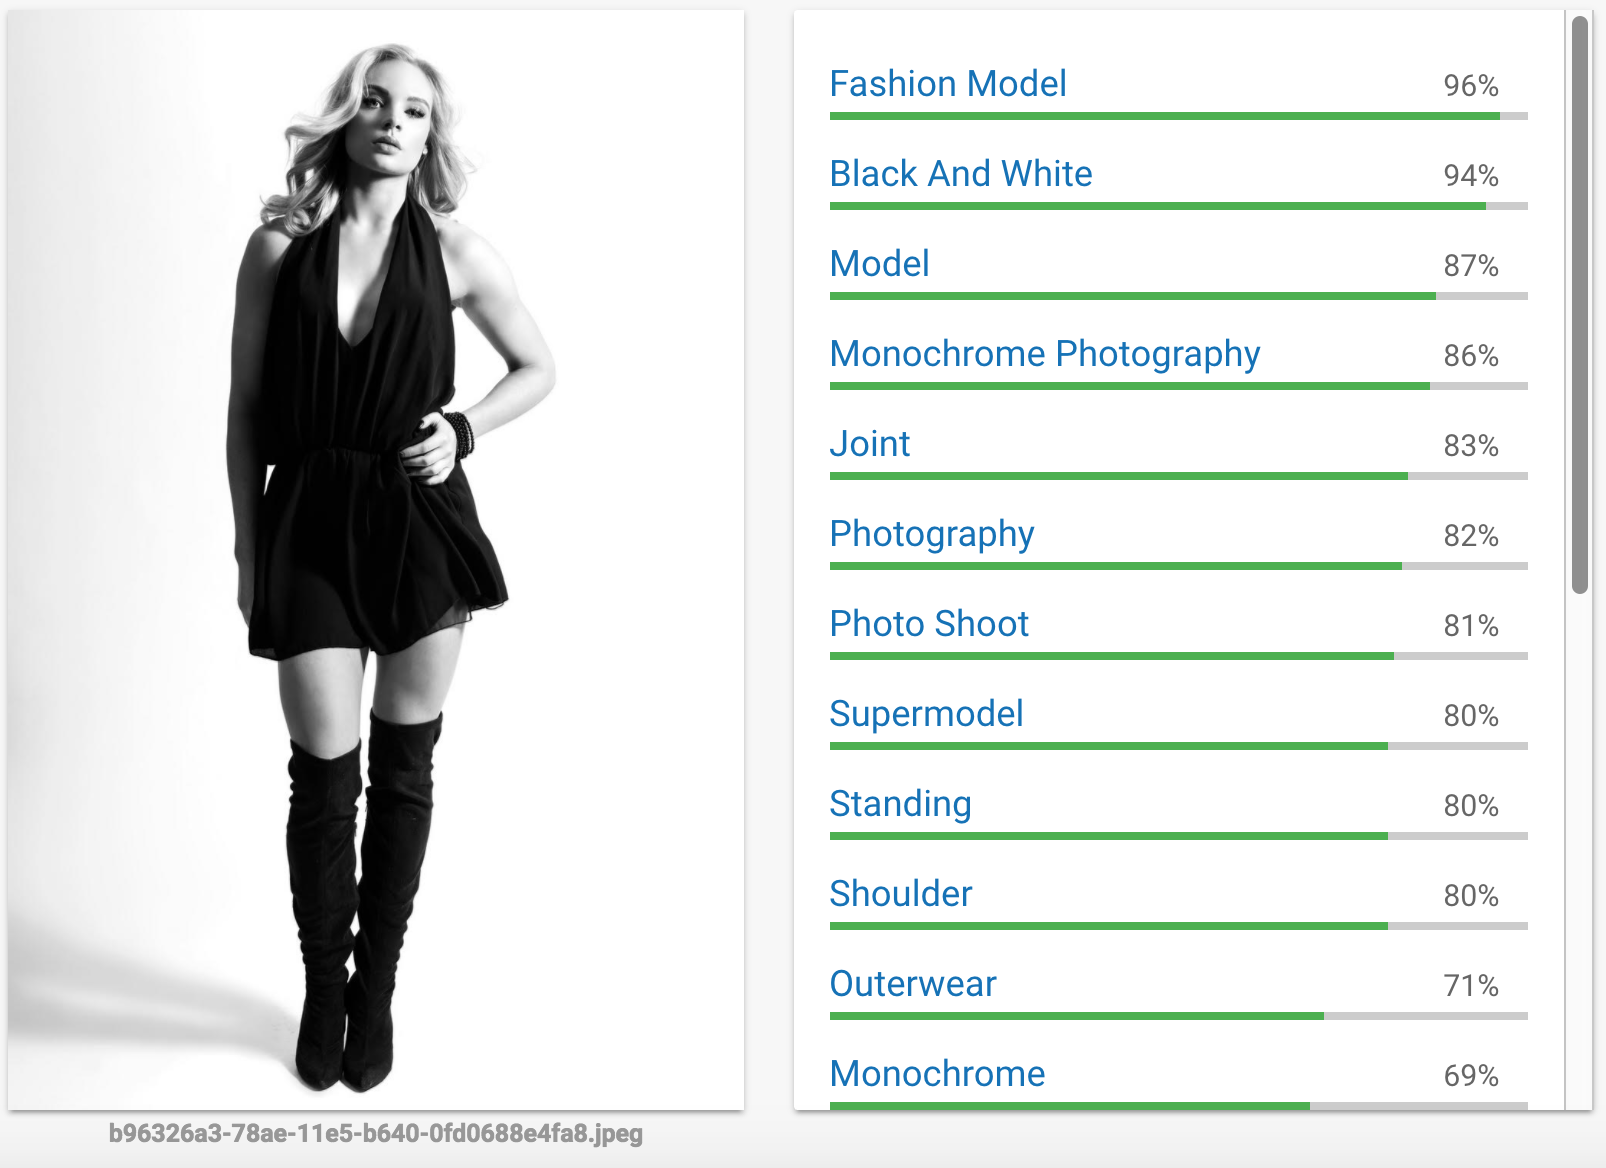
\includegraphics[width=0.8\textwidth]{images/google_vision_labels.png}
            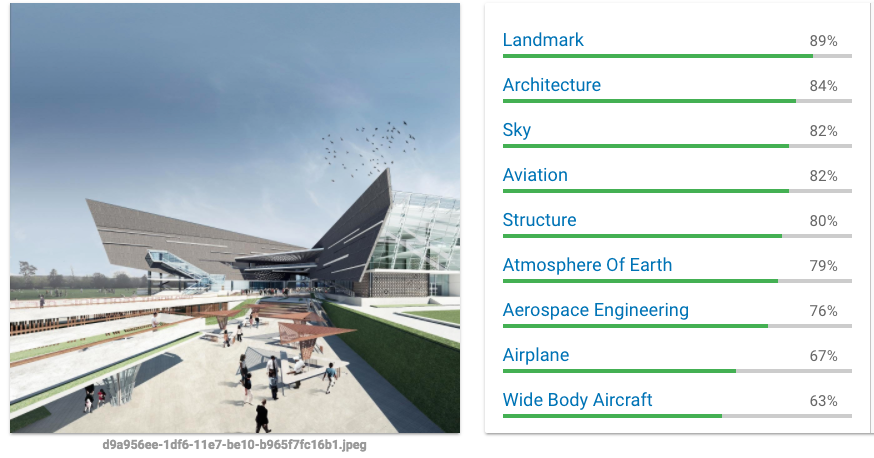
\includegraphics[width=0.8\textwidth]{images/google_vision_labels2.png}
			\caption{The labels identified by the Google Vision API on two of the contest participant's images.}
			\label{google_vision_labels}
		\end{center}
    \end{figure}

    % how are the labels used - what is the method performed on them? 
    Combining the identified labels and the vote data can provide information on user behavior. For instance it can be identified which demographic group of users like what kind of content, or the behavioral differences between two or more groups can be compared to eachother. Furthermore, this kind of information could be used to recommend new content in the platform to users which they have not seen before. Last but not least, it could be identified that which traits of participants contribute to more votes and engagement by users or certain user groups.  
    
    \subsection{Data structure and retrieval}
    % architectural overview
    In order to better understand the data, the data structure and the architecture of the Choicely platform is explained briefly in this subchapter. Most of the platform's data is stored currently in the Google Cloud Platform\footnote{\url{https://cloud.google.com}}, more specifically in Google Datastore\footnote{\url{https://cloud.google.com/datastore}} and Google BigQuery\footnote{\url{https://cloud.google.com/bigquery}}. Google Vision\footnote{\url{https://cloud.google.com/vision/}} is utilized as a computer vision service to gather the meta data for the contestants' images. 
    
    Google Datastore is highly scalable document database which is built on top of NoSQL technology \cite{google-datastore-overview}. By providing flexible storage, performant computing resources, encryption possibilities and high availability, the service can serve wide range of applications and various type of business data of companies \cite{google-datastore-overview}. Google BigQuery is a data warehouse for enterprise purposes, large-scale data storage, processing and analysis \cite{google-bigquery-overview}. Most of Choicely's data is stored in Google Datastore, however the computer-vision identified tags of the participants' images (Figure \ref{google_vision_labels}) are located in Google BigQuery at the present time.
    
    The data is structured into entities in both Datastore and BigQuery. There is parent-child connection between entities, which are key for the retrieval of some of the unique entities. For instance, contests belong to Users or Brands (as content providers), which are separate entities in the platform. Certain entities can be identified by multiple parent entities. Entities that have no parent(s) can be identified with their unique identifiers and indexed with some other fields. For example, users can be filtered by gender and age group, or unique identifier. 
    
    The data is generated by content providers, who create contests in the platform and users, who cast votes on their favorite participant(s) in the contests through one of the interfaces explained in Figure \ref{choicely_platforms}. The contest participants' images are identified automatically via the combination of Google Vision \footnote{\url{https://cloud.google.com/vision/}} and Google Cloud Functions \footnote{\url{https://cloud.google.com/functions/}} once they are uploaded to the database. Google Vision is another component of the Google Cloud, which provides powerful image analysis solutions for software developers \cite{google-vision-overview}. In this study, the usage of this component is limited to the classification of the content on the images as explained above.  Google Cloud Functions \footnote{\url{https://cloud.google.com/functions/}} are used to be able to automatically assign the labels to the images so that the manual work can be reduced to the least minimum. 

    Similarly to SQL join statements, the aforementioned identifiers and the parent-child relationship can be used to join list of various entities together. This property is used to aggregate and prepare data for the purposes of the analyses to be performed. Accordingly, the Contest, User, ContestVote, Vote and ImageLabel entities are joined together via their connections to construct the data structure displayed in Table \ref{association_analyisis_data}. This data structure establishes the basis of the Association Analysis, which is performed to address RQ3. 

    \begin{figure}[h] 
		\begin{center}
            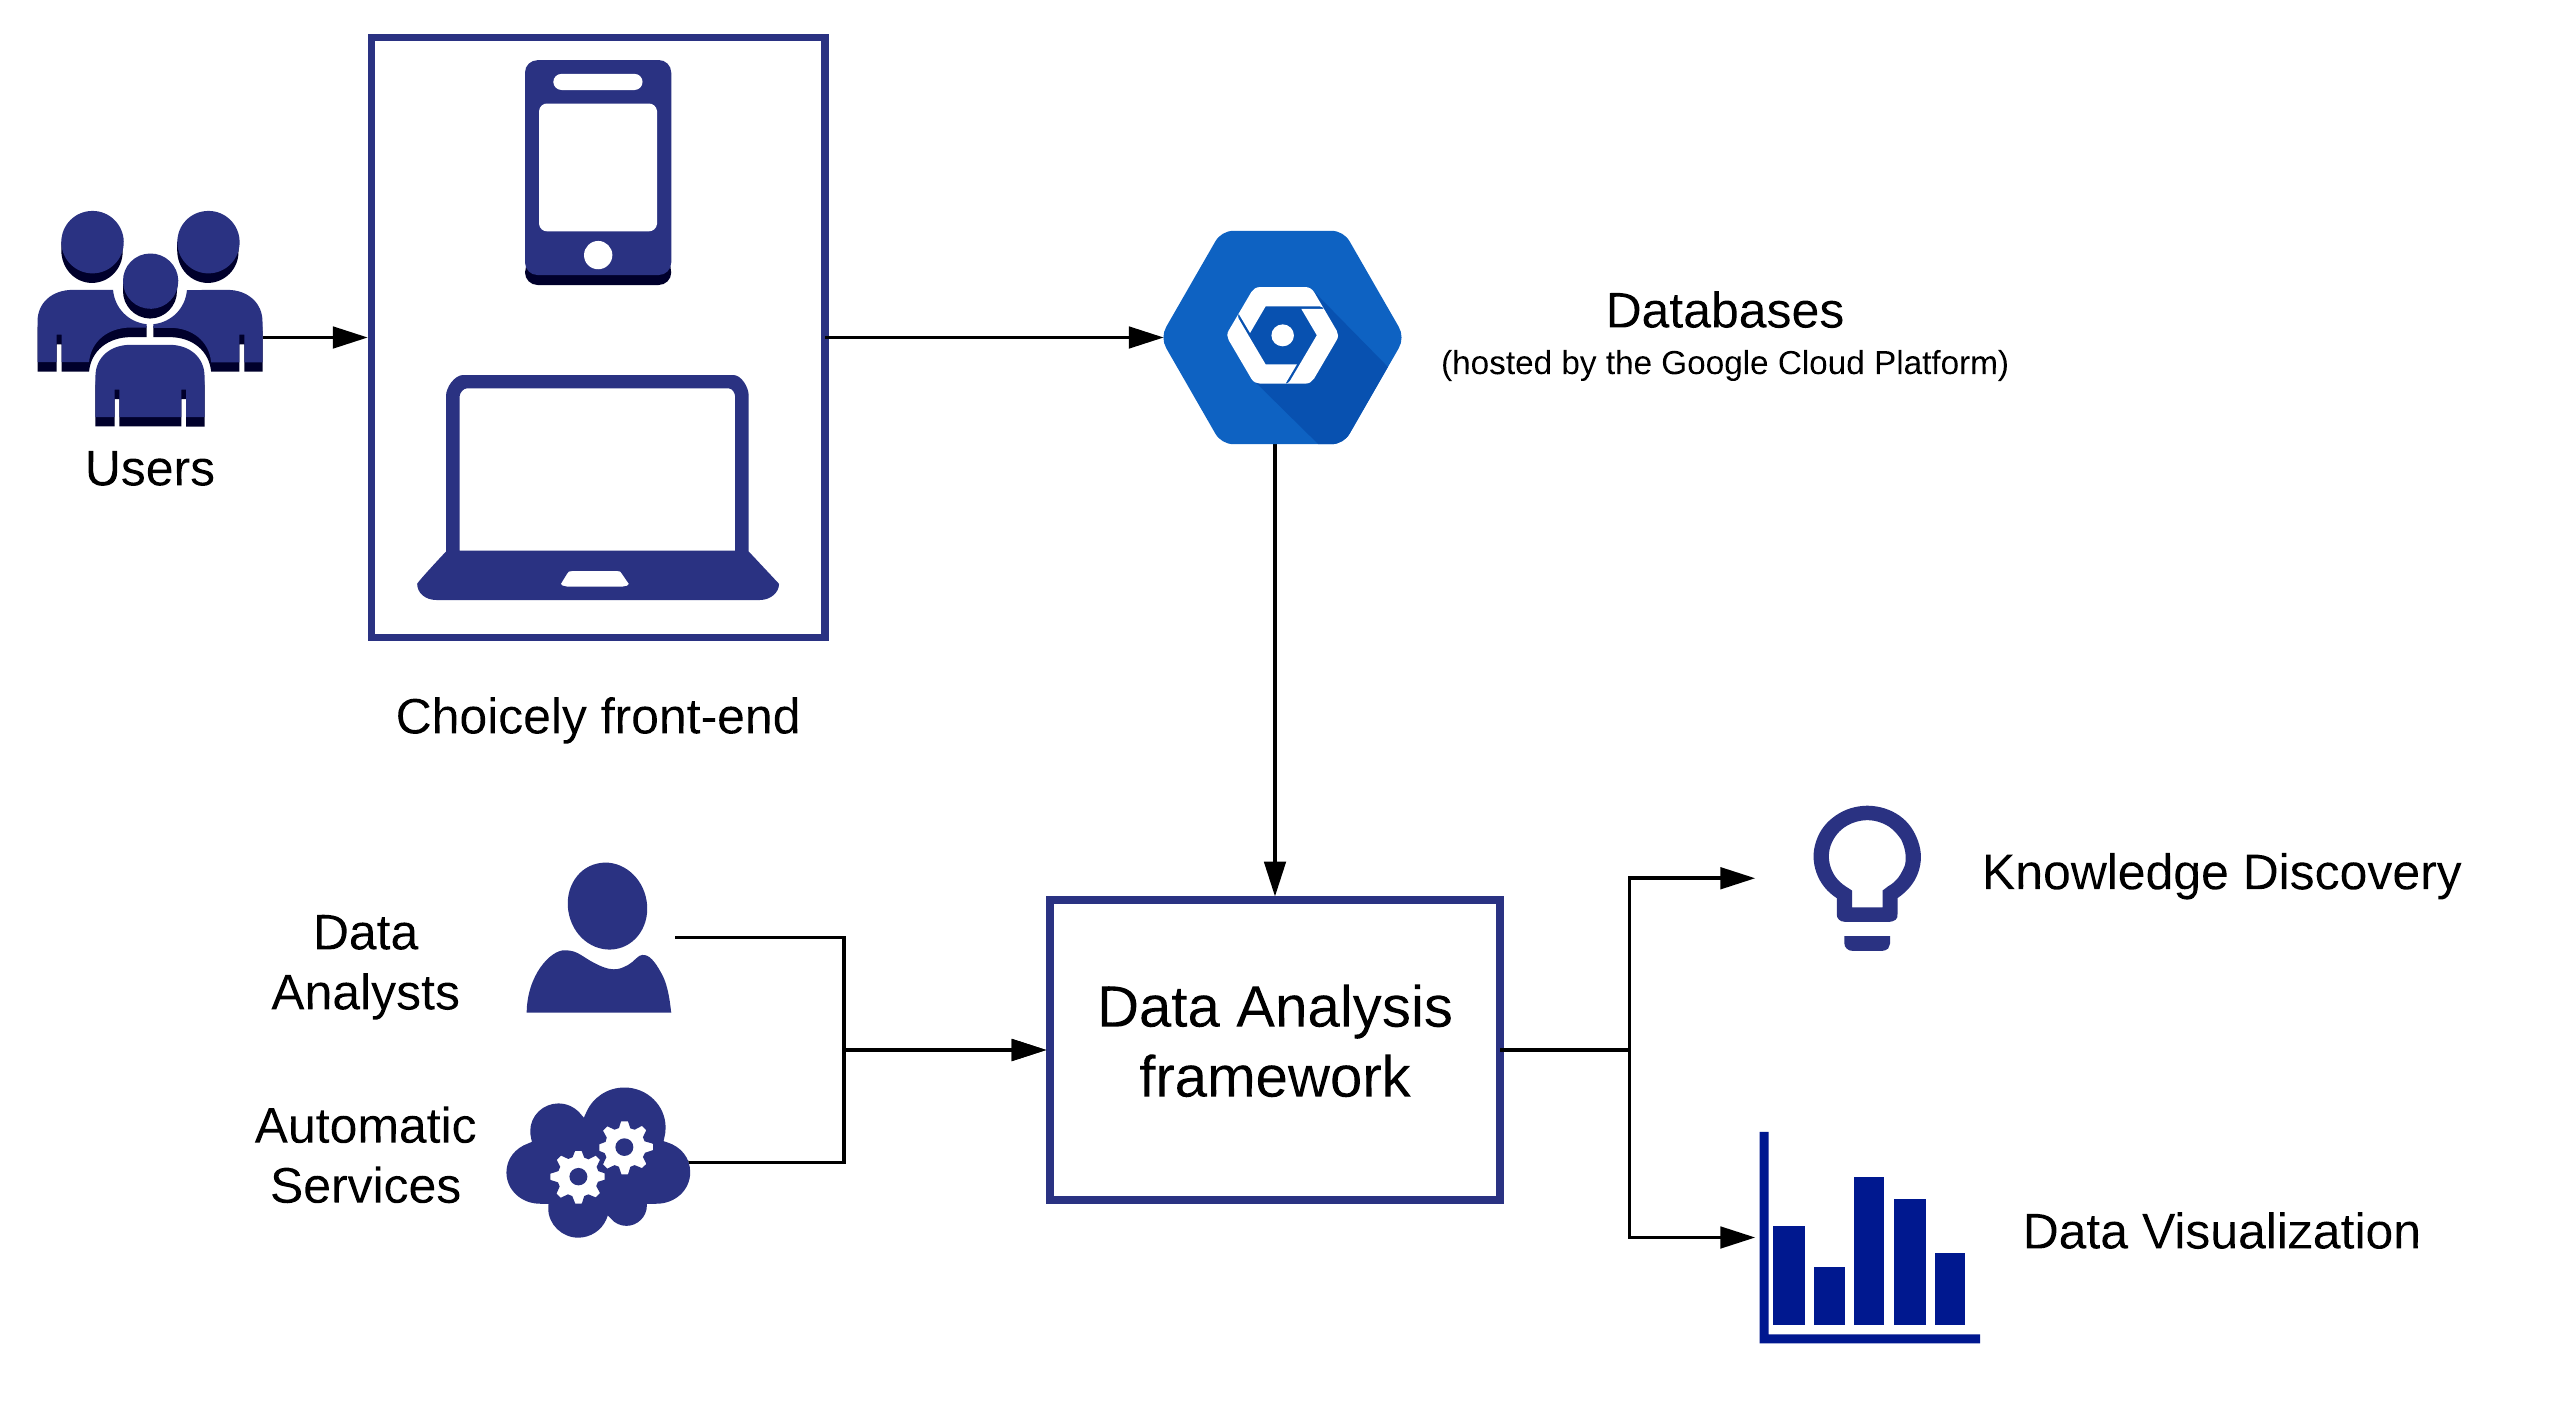
\includegraphics[width=0.8\textwidth]{Images/architecture.png}
			\caption{The brief architectural overview of the Choicely platform.}
			\label{choicely_architecture}
		\end{center}
    \end{figure}

    Figure \ref{choicely_architecture} displays the architecture of the Choicely platform on a high level. The Users of the system use the Choicely clients on their mobile or personal computer to create new contests or cast votes in the existing ones. 
    % From the point of view of this thesis work there are no significant differences between the two entitites, their role is simply to provide engaging content to a large number of users. Users then on the other hand participate in the contests by casting votes on the contest participants. 
    The Vote and Contest data is collected and stored to the databases that are hosted by Google Datastore. The data analysis is then performed by the Data Analysis framework, which is used by either a data analyst or an automatic service. This thesis work is devoted to establish the core functionality of this framework through this thesis work. Finally, Knowledge Discovery and Data Visualization is performed on the output of the framework. 

    % conclude why is this architecture interesting - point out nowadays it is common to have scattered data in multiple databases etc.
    % TODO
    
    % \begin{figure}[h] 
	% 	\begin{center}
    %         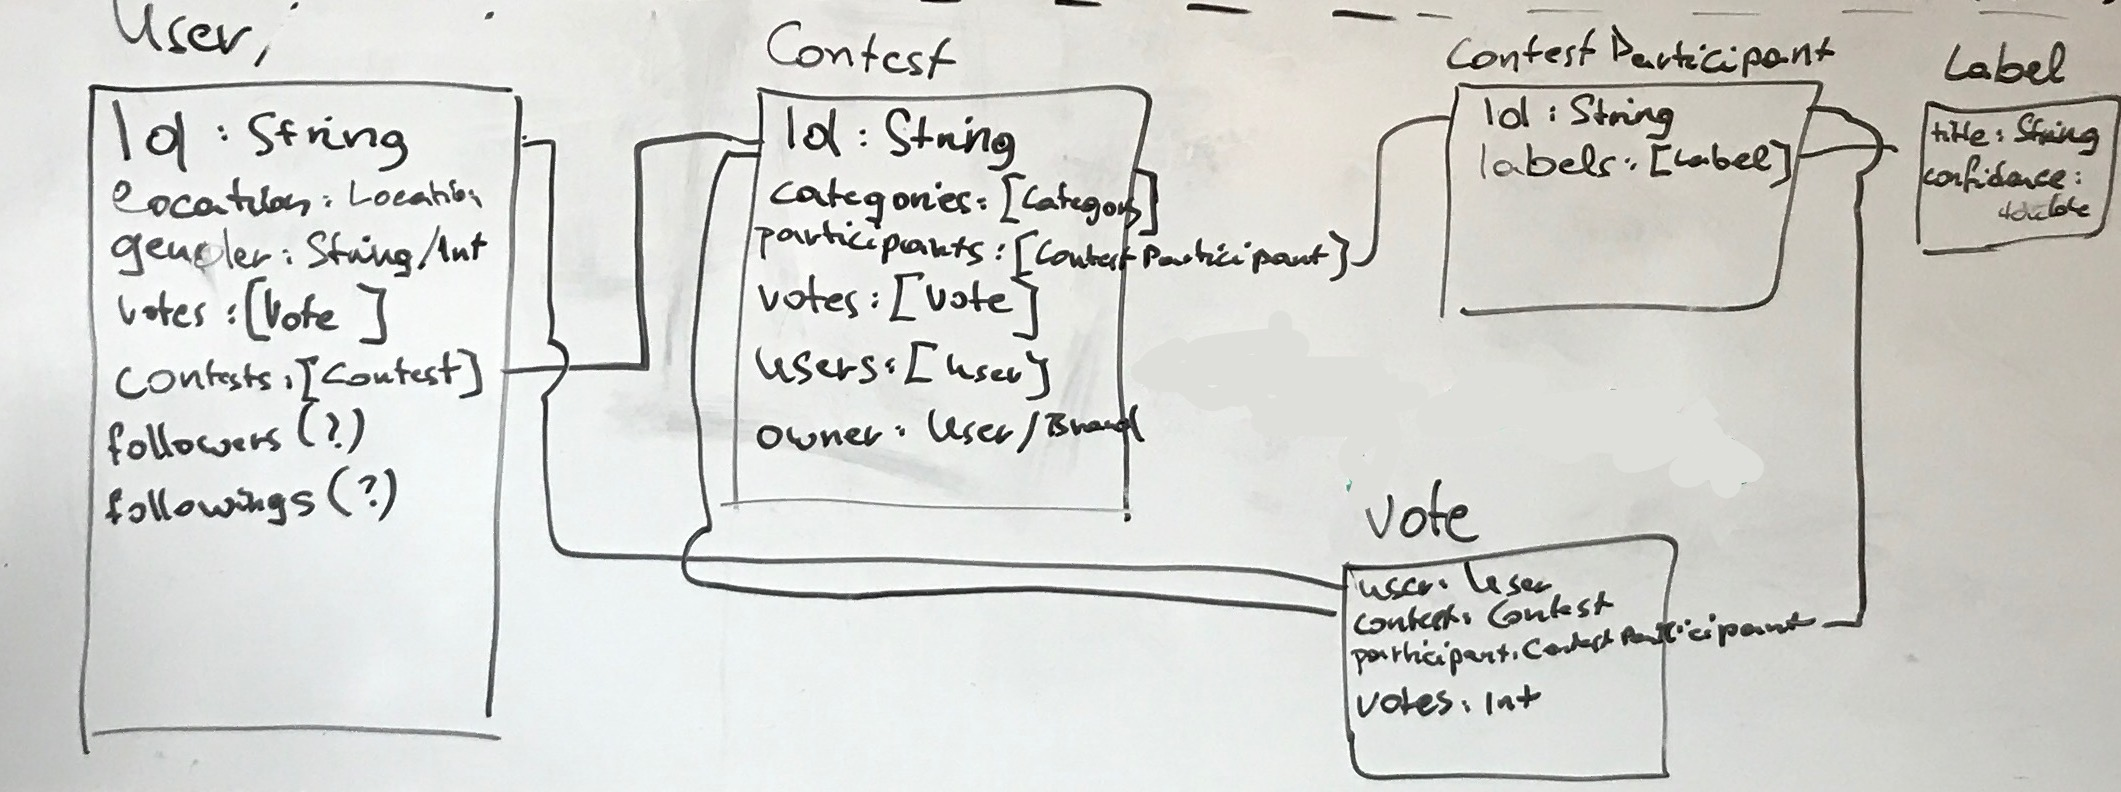
\includegraphics[width=0.8\textwidth]{Images/data_structure_whiteboard.jpg}
	% 		\caption{The structure of the data models of the Choicely platform.}
	% 		\label{choicely_data_models}
	% 	\end{center}
    % \end{figure}

    %\subsection{Knowledge Discovery and Data Visualization}
    \subsection{Applying the chosen methods}
    To answer RQ2 and RQ3 (presented in Chapter \ref{section::introduction}), the chosen methods presented in Chapter \ref{section::methodology} are applied in relation to Choicely's data. The paragraphs to follow elaborate a more in depth, what kind of data is used in case of the Choicely to answer the stated questions. On top of that it is explained, how the data was transformed in order to achieve the results. Data records collected before $1^{st}$ January, 2018 are used for the analyses. 

    % what is the goal of EDA? How is it used in this research? 
    The EDA fundamentally focused on two aspects of the data at hand: the user engagement in contests and the completeness of user profiles. In other words, the EDA is performed on the datasets extracted from the Contest, User and Vote entities in Choicely. This choice is done with the aim of addressing the research space of RQ2.  
    
    Contests have a few attributes which can help answering RQ2. To gain an understanding on how many users are typically engaged in contests, the number of unique voters is studied in comparison to the number of contests. The number of unique voters means the users, who have voted on at least one participant in a contest. This value can be retrieved for all contests in the platform. Contests can be filtered by their categories which is another approach towards finding answers to RQ2. Similarly to studying the number of unique voters over contests, the same metric is applied to all contest categories. By looking into how many users have voted in which kind of contests, one can get a grasp on the kind of contests that tend to attract more users.

    On top the number of unique voters, it can be studied what percentage of the users vote in more than one contest in a category. In other words, the return rate of users over categories can be studied to identify more engaging type of content. Accordingly, the Vote records are studied from the angle of voters and categories.

    To answer RQ3, Association Analysis using the Apriori algorithm is performed. In order to be able to execute the analysis, some preprocessing has to be done. The list of labels extracted from the participants in the contest are listed for each transaction alongside with the voters' demographic data. In other words, the data has to be transformed such that the input contains rows of the voters' demographic attributes and the computer-vision identified labels from the participants' images. In order to achieve this, the User, Contest, ImageLabel and Vote tables are joined together. The retrieved data is combined as shown in Table \ref{association_analyisis_data}. This data structure is adequate to perform the analysis on.

    \begin{table}[]
        \centering
        \begin{adjustbox}{width=1\textwidth}
            \begin{tabular}{l|l|l|l}
                gender & age group & country & labels \\
                \hline
                female & 25-34 & fin & ['fashion model', 'hair', 'model', 'beauty', '...] \\
                male & 18-24 & fin & ['dark hair', 'hair', 'model', 'smile', '...] \\
                male & 65+ & fin & ['fashion model', 'hair', 'shoulder', 'beauty', '...] \\
                female & 18-24 & swe & ['fashion model', 'hair', 'model', 'beauty', ...] \\
                male & 18-24 & hun & ['beauty', 'blond', 'human hair color', 'model', ...]
            \end{tabular}
        \end{adjustbox}
        \caption{The format of the data used for Association Analysis (the records dispalyed in the table are only examples).}
        \label{association_analyisis_data}
    \end{table}

    After transforming the data, the Apriori algorithm is applied to calculate the itemset supports. This can be done on arbitrary amount of vote transactions as long as they have been transformed to the desired format. However, there are certain cases when it makes sense to perform the analysis. For instance, the analysis can be performed 

    \begin{enumerate}
        \item on transactions of a single contest: this way contest organizers get a chance to analyze their engaged audience and seek the tendencies in their behavior,
        \item on transactions extracted from the complete dataset: this way one can attempt to find patterns in how users behave on the system-level,
        \item on transactions of a targeted group of users: this approach allows to understand the preferences of a desired group of people across multiple contests,
        \item on transactions of a single user: this way the behavioral patterns of the individual user can be studied and analyzed. 
    \end{enumerate}

    It would be interesting to take a look into all of these aspects, however the scope of this thesis work limits the analysis to be performed. On top of that, items 3 and 4 might go into "too personal" directions, hence interfere with privacy issues and raise ethical concerns. In order to keep the scope of the analysis on a reasonable size, Therefore, items 1 and 2 in the above list are taken in the analysis and the rest are discarded. 
    
    Using the approach explained above, the support of the itemsets extracted from the labels can be calculated. The support in this case tells the percentage of votes, which were casted on a desired itemset. For instance, $S(\{"beauty", "blonde"\}) = 0.6$ would mean that $60 \%$ of all votes were casted on participants whose images contained the $\{"beauty", "blonde"\}$ itemset. Likewise, if the list of vote transactions is filtered by one of the demographic attributes, the same can be said for the investigated group of users. 

    To control the algorithm's runtime is not too long, the $minsup$ value is set to $0.05$, which corresponds to $5 \%$ support. This means that all itemsets, that have smaller support than this value for all demographic groups, are pruned during the progression. On top of reducing runtime, this threshold is set to eliminate less interesting itemsets and keep only the interesting ones on the output.

    The result of the Apriori algorithm then can be collected into a table displayed on Table \ref{itemset_supports_format}. This table shows the itemsets as rows and the targeted group of users as columns. The values in each columns correspond to the support values of the itemsets for the given group of users in the set of transactions that was feeded to the algorithm. 

    % TODO consider if the next paragraph is needed at all
    % Note that despite the values in the rows are probabilities, their values do not have to sum up to $1.0$. This is because each value in the table tells the probability, that a randomly selected transaction will contain the itemset (row), given that the vote was casted by a person who belongs to the target group (column). In other words, the probabilities of the itemsets for the demographic groups are independent from eachother.

    \begin{table}[]
        \centering
        \begin{adjustbox}{width=1\textwidth}
            \begin{tabular}{l|c|c|c|c}
                X & $S(X|gender=male)$ & $S(X|gender=female)$ & $S(X|gender=other)$ & $S(X|gender=not\_specified)$ \\
                \hline
                $\{"beauty", "blonde"\}$ & $0.6$ & $0.8$ & $0.15$ & $0.25$ \\
                $\{"cat", "fluffy", "cute" \}$ & $0.6$ & $0.1$ & $0.5$ & $0.0$ \\
                $\{"sea", "photo shoot", "model"\}$ & $0.0$ & $1.0$ & $0.33$ & $0.65$
            \end{tabular}
        \end{adjustbox}
        \caption{The output format of the Association Analysis comparing genders, where X is the itemset and S is the support (the records dispalyed in the table are only examples).}
        \label{itemset_supports_format}
    \end{table}

    In order to better understand the results of the Association Analysis, first a single contest (Miss Suomi 2017\footnote{\url{https://choicely.com/contest/164f52c7-9df8-11e7-b3c9-d1a0f88250ad}}) is looked at more carefully. By looking at a single case study, the results can be analyzed and interpreted in a smaller scope and hence be understood easier. Secondly, the results of the analysis performed on the system-level are presented and interpreted. This approach is chosen to demonstrate the capabilities and the potential of the technique in both smaller and larger datasets.

    The Miss Suomi 2017 contest has been hosted in the Choicely platform late September, 2017. Having engaged $26 200$ users, it is the third biggest contest in the platform at the time of performing the analysis. There are $10$ participants in the contest, who were photographed while dressed in white cocktail dresses on a shore of a lake or sea. Each photo has one and only one participant. Each participant has only one and only one photo in this contest. 
    
    Depending on how many individual participants the chosen transactions target, the number of itemsets (hence the number of rows) grows rapidly. Also the number of demographic groups (hence the number of columns) may differ depending on which the property is used from the users' profile. Essentially, the number of categorical groups for genders can go up to 4, for age groups up to 7 (see Table \ref{user_profile_fields}), but many more for location-based groups. As a conclusion it can be said that despite the supports are obtained, most likely their number will be too overwhelming to look at and analyze.

    % Finally, Co-Clustering is utilized on the calculated supports 
    For this reason, the Co-Clustering method is used to identify which itemsets or demographic groups show similarities. The method is applied on the output of the Association Analysis displayed in Table \ref{itemset_supports_format} in order to explore the underlying structure behind the itemset supports and demographic groups. The implementation is done with the help of the bicluster module \cite{scikit-bicluster} of the popular scikit learn package \cite{scikit-learn}. The Spectral Co-Clustering class is used for the analysis, which proposes to pinpoint biclusters with higher values than others according to the documentation \cite{scikit-bicluster}. 

    Using this approach, the clusters that are similar to eachother are going to be organized close to eachother. The algorithm's input requires a \textit{k} value, which corresponds to the number of clusters to seek. The cluster labels are attached to each row and column respectively, which suggests the itemsets and demographic groups that belong to the same cluster. In the performed analyses, the k value of the Co-Clustering algorithm is set to $4$. 

    By knowing the clusters, one can conclude if there are tendenies among demographic groups in terms of behavior. For instance, if the age group 65+ and 0-17 would be assigned in the same cluster by the algorithm, that would prove the similar behavior of the users in these two groups. In other words this would mean, that the certain kind of content leads to the engagement of both of these groups, but not necessarily the others. This can be valuable information to marketing professionals in the situation, when they wish to target a specific group of discussion. The demographic traits could be further combined in theory (e.g. male teenager users from Finland), however this deep analysis is out of the scope of this thesis work. 
	
	\section{Discussion}
	\label{section::discussion}
	% variance in user data (especially in the digital footprints)
Based on the reviewed literature, there is no common understanding on the term of user data among researchers. While demographic data is very well understood, digital footprints (data gathered during the usage of a software) are less commonly studied in the field. It is clearly identified that the careful utilization of user demographic data and digital footprints, software service providers and researchers can retrieve previously unknown information about users' behavioral characteristics. 

% no common understanding 
Users' demographic data and digital footprints are not usually brought under the same hood, are often vaguely defined and sometimes are studied separately. By introducing the concept of user data, a common ground of understanding is set for researchers of the future. As a scientist in this area, it is essential to understand the variety of user data in terms of availability and format. Depending on the software at hand, the data generated by digital footprints varies, while user demographic data is more uniformed.

Access to demographic data in the present time seems to be getting easier for researchers. Social networks already have standard ways of helping users to authenticate themselves while using other services (in other words use their social network credentials to use other services). Taking advantage of this, businesses can get access to rich demographic data of their user base easily. This fact creates a research space for studies, that have not been possible in the past. 

% why are these researches interesting? What do we learn from the society by performing analysis on user data? 
The reviewed research papers demonstrate how others have utilized Data Mining and Machine Learning methods to reveal patterns or behavioral characteristics of users. The proper application data analysis methods allows us researchers, to learn more about the society as well as human behavior, which was not possible previously. This information is essential for business operations, because it gives insights on the user groups, their preferences and what kind of content keeps the audience engaged. In conclusion, the interest and relevance of applying computational methods in this area is proven.

The set reviewed studies show, that Natural Language Processing and Supervised Machine Learning techniques are the most common approaches for conducting research on user data. The encouraging results achieved by other researchers prove the relevance of computational techniques applied on user data in a wide range of development areas, such as banking, social media, online movie databases, user portfolio analysis, to name a few. This suggests that computational methods are versatile enough to be applied in various domains. However, as every software and dataset is unique in some sense, there is not a single method that could be consdered as a silver bullet to solve problems. 

In the past audience engagement was hardly possible and knowing the interests demographic user groups was challenging. In the present time, access to this information can facilitate research, business processes, help determining the future content, analyze trends and understanding target groups of particular services better. In sum, modern Data Mining techniques created the potential to study human preferences and behavior from a different angle.

The results from studying the Choicely platform demonstrate an actual realization of the user data concept. The platform incorporates demographic data of its users as well as digital footprints of the software's usage. The nature of the platform is interesting, because users' engagement, voting trends and favor towards contest participants can be extracted from the data. Using the developed data analysis framework, contest organizers can analyze the engagement summary after a contest is over in a new way. 

The developed tools can not only pinpoint the content that is more appealing to users, but also reveal the tendencies shown by different demographic groups. This provides the potential for developing customized services and content for the groups, which then leads to better user experience while interacting with the platform. For example, if younger users show more interest in sports, while elders in traveling, customized content recommendations can be made to them, either in the Choicely platform or in external sites. Furthermore, this knowledge can also contribute to better product design and marketing, because the quantified results can confirm preliminary hypotheses concerning users' personal desires. 

% Evaluation of the chosen research methods
The chosen methods for the practical part of this study help the company to understand the data at hand better, as well as to provide better services to their customers. The methods used in this study are relevant tools towards answering the research questions, however their limitations were also demonstrated in the study. Hence it is important to know the pros and cons of these methods and think critically about their applicability and relevance to problems. Therefore, the chosen methods are retrospectively reviewed in the scope of this study in the paragraphs to follow.

EDA has provided great access to statistical measures as well as visualization tools to explore the data. Through this study it can be seen great technique for getting a grasp on what the data at hand looks like and what it contains. This method provides the possibility of laying down initial hypotheses and conceptualizing the "big picture". Looking at the data in general is a good idea not only to explore, but to understand how observations relate to eachother and what the connections between them are. Despite being a useful technique, EDA is limited to this only purpose and cannot answer complex questions, nor it can identify underlying structure or patterns in many cases. Last but not least, EDA can reveal also the potential biases in the data with the choice of proper visualization and statistical measures. In this study EDA for instance pinpointed the fact that many contests are considerably small in terms of voters and hence helped enhancing the results in later stages. The finding that some contests did not have proper meta-data and labeling was also obtained through this research method. Last but not least, the technique also revealed which type of contests in the platform have more data to work with, which led to better and valid results. 

By performing Association Analysis some preliminary assumptions in the EDA phase have been confirmed. More importantly, the calculation of the itemset supports have contributed towards answering the research questions in more details. Based on the results it can be concluded, that contests in the "beauty" and "fashion" categories create higher engagement than others, which may be explained by the history and the customer base of the firm. Nevertheless, it seems that contests where participants are human beings are more attractive to voters, whereas abstract objects or places appear less interesting to the audience. 

Itemset supports on their own do not necessarily tell all of the interesting information about the engagement of the audience. The lifts of the itemsets are more interesting to look at and can enhance the provided information with more interesting and meaningful insights. 

It was identified, that studying the generated itemsets in a single contest is possible and can assist the organizer to retrospectively analyze the content which has engaged the audience. Using this data, different demographic groups and their preferences can be compared and analyzed. Due to the fact that the biases in the data enlarge on the system level, it is difficult to derive valid results using the current methods and data on a larger scale. It would be hence important to enhance the quality of the data over the contest or to use an even subset of data for such purposes.

This method also contributed to identify, that the labels assigned to images by Computer Vision are very similar to eachother. This led to similar support values in some cases and somewhat biased results. The reason behind this is the fact that chosen Computer Vision tool recognized only the main objects on the images and omitted the details. It would be interesting to enhance the image labels with more specific tags or other meta data (either manually or automatically), that tell unique features of the participants, then perform the same analysis and compare the results. This approach could point out more details concerning which detailed features of participants lead to more attention and engagement from users.

The large number of generated itemsets via this technique also makes the readability of the results challenging. When the generated itemsets grow over certain size (typically 2-3 items), the number of output items is too high to analyze manually. The Co-Clustering technique addresses this challenge well by clustering the matrix of itemset supports and the demographic groups. Through this technique, the itemsets and demographic groups whose structures are similar can be identified and analyzed more carefully together. The results of this approach also can make suggestions for demographic groups, who share similarities in terms of their voting behavior.

One of the challenges with the Co-Clustering method is to choose the number of clusters. For the time being, there was not a single good way of suggesting the best value for this value, because the best match for the number of clusters depends on the size of the dataset (in terms of itemsets and demographic groups) and the underlying structure of the data. Nevertheless, it seems that trial and error works considerably well in this case, but interpreting the results is often not evident. It would be interesting to develop the solution towards a direction, where this challenge is addressed.

The assignment of the cluster labels in the current implementation could be questioned. The fact of assigning one cluster to every row and colum puts a limitation to the outcome. A large number of cells do not belong to any clusters, because the algorithm assumes a block-diagonal structure, which might not be the case in this kind of dataset. In order to improve on that, it would be a good idea to apply more complex and flexible Co-Clustering algorithms for the analysis of the underlying structure. Such algorithm could consider cell-wise comparisons and cluster assignments, which would be more robust in identifying homogeneity of items inside clusters. 

Through the results it can be seen how differences in the behavior of demographic groups are revealed. For instance, through the application of the methods it is speculated that users in the Choicely platform can be seen as specialists and generalists. Furthermore, the data suggests distinctions between the younger end elder generation as well. 

Biases in the data limit the conclusions and the viability of the results and raise threads to their validity. To address this issue, there is a need for a more careful evaluation on the statistical significance of the results. The dataset could be enhanced with more reliable and validated data. One could carry out a structured data collection from a chosen sample of users to ensure the validity of the collected data. Another angle on this topic is that the Choicely platform is rather unique in nature compared to social media sites for instance. Therefore the results obtained in this study may be difficult to reproduce in other online software platforms.

% Privacy and ethical concerns
Privacy and ethical concerns are interesting for many reasons to discuss through the scope of this study. Undoubtedly, the recent technical evolvement has brought many challenges with respect to human rights and data protection, hence there is a need to lay down a common standard in the European Economic Area (EEA). The General Data Protection Regulation (hereinafter GDPR) \cite{gdpr} is being issued on 25th May 2018, which regulates the business and data processing activities by protecting personal data through its novel standards all over the world. According to the regulations, personal data means any kind of information through which the natural person (or data subject, who has generated that data) can be identified \cite{gdpr}. 

The data analysis activities performed in this study are operating on personal and sensitive data, however the results do not reveal any piece of that data. Based on the results of the audience engagement presented in the present research, there is no possible way to identify individual data subjects. The results only show the extraction and statistically significant information about the collected data, but fully hide the individual's personal data. In terms of the GDPR, these activities are called "profiling" \cite{gdpr}. As by Article \cite{gdpr}, the data subject has to be clearly informed about the purposes and goals how his or her generated data is being used. Many other important aspects, such as portability, erasure or automated decision making are addressed over multiple articles (12-23) concerging the rights of the data subjects and the responsibilities of the processor \cite{gdpr}.

In terms of the case company this means, that the purposes of any data processing tasks should be clearly stated and communicated to users. A standard and convenient channel to forward this information to the platform's users is the company's privacy policy\footnote{\url{https://choicely.com/about/privacy}}, which already contains a list of points in this topic. Nevertheless, as the results and methods of this study are being added to the platform, this list should be extended by clearly expressing the purposes and goals of data collection and analysis.

% self criticism, what would I do differently? 

	\section{Conclusions}
	\label{section::conclusions}
	% what are the main messages and takeaways? 
User data is widely collected and commoly used for research purposes as well increasing business value of services. The willingness to give this data from users' perspective is present, as many social media sites create a reliable and convenient hub for such repositories. As a consequence, businesses and researchers can easily get access to rich demographic and software usage data through the interfaces of socila media platforms. Furthermore, these platforms serve the purpose of convenient authentication and integration to other services, which is highly appreaciated by the users. On top of that, the software service providers get easy, quick and reliable access to demographic information about their users. 

Despite its wide availability, the concept of user data is not commonly used in the literature. Nevertheless, numerous studies were conducted in the past - mainly via social media websites - to analyze engagement and trends on how users behave in an online environment. The research topics mainly resolve around what kind of content is attractive to them or how they communicate with eachother in the online softare. One of the challenges in this area is, that every software platform is unique, therefore there is not a single way of studying these aspects. Secondly, the data at hand can differ from platform to platform, nevertheless it is commonly too large to analyze using human labour. For this reason, various Data Mining and Machine Learning techniques were utilized by the scientific community to enhance and analyze the data at hand. 

Through this research it was revealed, that while user demographic data is often well established, digital footprints are very domain-dependent in nature. It is concluded that the both sides of user data is necessary to analyze user characteristics and behavior. The combination of computational methods and such data has been already utilized in various areas, such as banking, studying and predicting movie ratings, social media studies and enterprise social networks. This observation proves the relevance and the wide applicability of this research area. Depending on the domain, various tools and methods, such as computer vision, machine learning, association analysis and natural language processing techniques are available, but none of them is a silver bullet for every dataset. 

The Choicely voting/audience engagement platform is an excellent specimen for a software service, where user data is utilized. The aim of this research was to study the user data that is collected by the Choicely platform. The study analyzes the type of content that appears more engaging to users and investigates the voting behaviors of different demographic groups. 

The user data at Choicely is two folded. Users from all over the world log in to the platform, typically using one of their social media credentials to authenticate their identity. As a result, their personal profiles are created in the Choicely platform with their demographic data pre-populated, which establishes one half of the data. The second half of user data is generated by users while using the software. In case of the Choicely platform this means vote transactions on the participants of the contests. 

Each contest participant can be connected to a single image in the platform. The contents on the images varies and generally speaking, there is no standard of labeling the images with meta data for analysis purposes. As a result, analysis on the vote transactions is difficult, because it is not possible to know the type of content users find engaging.

To tackle this problem, Computer Vision (using Google Vision) was integrated to the platform. This technology can reliably assign meta data to the images concerning thier content automatically, whenever they are uploaded to the platform. The vote transactions hence can contain not only on who voted on which participant, but also what the content on that participant's image is. The combination of this data together with the users' demographic data opens up the possibility for a more sophisticated data analysis on the data, in order to study engaging content and users' behavior in the platform. 

To enhance the firm's business package, the basis of a data analysis framework were established. Association Analysis is utilized to extract the support values of the itemsets that appear in the vote transactions. 
The vote transactions can be studied from multiple angles, however this study was limited to single contests and system-wide analysis. By studying transactions of a single contests organizers can evaluate, which labels tend to be more engaging to different demographic in the contest. Furthermore, this methods provides room for analyzing differences between groups as well as itemsets that appear in the contest. The system-wide analysis can reveal the same on a larger, global scale from a richer dataset. 

To computationally identify patterns and the underlying structure of the itemset supports, the Co-Clustering is used. The Co-Clustering is performed on matrix of itemset supports by demographic groups. This approach provides a reliable way to identify which demographic groups and itemsets tend to behave similarly in the data. As a result, engaging content that are specific to groups can be pinpointed, differences in the voting behavior between groups of users can be revealed. 

The results show that there are certain contest categories, which have hosted many more contests, hence have got more engagement than others. The Exploratory Data Analysis revealed, that there is a high number of very small contests. Deriving from this, only a fraction of the whole dataset is actually ready for complex data analysis, because the rest simply does not have sufficient amount of data to analyze. 

The Association Analysis on the itemsets recognized by Computer Vision reveals some interesting insights on the kind of content, which is more engaging to users. One of these findings is, that the contests where participants are actual people appeal to voters more than objects or other abstract concepts. Secondly, objects that appear in the foreground of the images might have more impact on the voting trends than the background or the surroundings, but there is no clear support for this claim. The results also reveal that Computer Vision in this research is useful to identify overall concepts of the images, however it fails to recognize smaller details on the pictures. 

Last but not least, the Co-Clustering approach was successfully used to pinpoint similar demographic groups and itemsets in the vote transactions. This technique provides a robust way to analyze behavior of demographic groups of users and pieces of content. However, this method has not proven useful on the system level, because the data in the platform is often incomplete. More particularly, the demographic data is often missing for many of the users and the assigned labels to the images are often share many similarities in contests. 

% future work
Future work could address on enhancing the quality of the data. The validity of the results in this study could be elevated applying these techniques on a more carefully selected and tested dataset. Future work could also build on top of the results of this study, for example a content recommendation system could be built using the results of Association Analysis and Co-Clustering. It would be also interesting to see the chosen methods performance in similar software platforms, particulary in social media applications. 

Due to the fact that user data involves a large set of personal data, there is an emerging need in studying and establishing standards for the research community. Future work could elaborate also more in-depth on the ethical concerns when conducting research with sensitive user data. Furthermore, it would be a interesting to approach this area not from only computer science, but human behavior point of view. Finally, the application of Data Mining and other computational techniques to facilitate studies focusing on psychology and human behavior would be another stimulating direction for researchers. Conducting more studies in this area would further deepen our understanding on human behavior, preferences as well as gender and cultural differences.     

\pagebreak

% TODO remove the next line when the thesis is completed
[Overall \total{citnum}\ references]

\nocite{*}
\bibliographystyle{tktl}
\bibliography{references}

\lastpage
\appendices
\pagestyle{empty}

%\internalappendix{1}{Model ABC}
%
%The appendices here are just models of the table of contents and the presentation. Each appendix 
%usually starts on its own page, with the name and number of the appendix at the top. Each appendix is paginated separately.
%
%In addition to complementing the main document, each appendix is also its own, independent entity. 
%This means that an appendix cannot be just an image or a piece of programming, but the appendix must explain its contents and meaning.

\end{document}